\documentclass[12pt,a4paper]{article}
\usepackage{ctex}
\usepackage{minted}
\usepackage{fancyhdr}
\usepackage[left=0.8in,right=0.8in,top=1in,bottom=0.9in]{geometry}
%\usepackage[total={6.5in,8.75in},
%top=1.2in, left=0.9in, includefoot]{geometry}
\usepackage{lastpage}
\usepackage{color}
\usepackage{graphicx} %插入图片
\usepackage{amsmath} %数学公式处理 align环境
\usepackage{setspace} %行间距
\usepackage{lmodern} %下行的使用需要这行
\usepackage[T1]{fontenc} %用于处理下划线等输出
\usepackage{textcomp} %\textasciitilde中划线 \textunderscore下划线
\usepackage{array} %使用表格的p{2cm}<{\centering}需要
\renewcommand\arraystretch{1.5} %设置表格的高度为1.5倍
\usepackage[pdfstartview=FitH,
CJKbookmarks=true,
bookmarksnumbered=true,
bookmarksopen=true,
colorlinks,
pdfborder=001,
linkcolor=blue,
anchorcolor=blue,
citecolor=blue,
]{hyperref} %实现目录和章节的超链接
\hypersetup{hidelinks}

\usepackage{chngpage} %使用adjustwidth环境偏移整个块 
\usepackage{cite} %引用bib中的文献


\pagestyle{fancy}
\fancyhf{}
\fancyfoot[RO,LE]{\thepage}
\renewcommand{\headrulewidth}{0pt}
%页眉横线宽度

\newcommand{\li}{\underline{\hspace{0.5em}}} %用于输出下划线
%\setboolean{@twoside}{true} %从oneside转换为twoside,这样才能有单数页和双数页码


\begin{document}
\title{Unix Socket Programming}
\author{邓岩\footnote{www.dengyan.net} \\ 837123564@qq.com}
\date{\today}
\maketitle
\thispagestyle{empty}
\newpage

\tableofcontents

\newpage

\setminted[c]{
			   breaklines,
			   %breakbefore= ,
			   %breakanywhere,
               linenos, %行号
               numbersep=10pt, %行号与代码距离
               autogobble, %去掉前两列
               %frame=lines, %边缘线
               framesep=5pt, %代码与框架距离
               %以下选项需要加在环境选项中才有效
               xleftmargin=2em,
			   %xrightmargin=0em,
			   %mathescape,
			   breakbefore= ,
}

\section{{\color[rgb]{0.2,0.4,0.6}前言}}
\subsection{头文件}
\begin{minted}{c}
// /Users/dengyan/ClionProjects/Linux/linux.h
//
// Created by 邓岩 on 09/03/2017.
//

#ifndef LINUX_LINUX_H
#define LINUX_LINUX_H

# include <sys/types.h>
# include <ctype.h>
# include <stdio.h>
# include <stdlib.h>
# include <unistd.h>
# include <errno.h>
# include <string.h>
# include <mach-o/getsect.h>
# include <pwd.h>
# include <grp.h>
# include <utmp.h>
# include <sys/stat.h>
# include <fcntl.h>
# include <sys/uio.h>
# include <setjmp.h>
# include <sys/time.h>
# include <sys/times.h>
# include <sys/utsname.h>
# include <time.h>
# include <utime.h>
# include <dirent.h>
# include <libgen.h>
# include <signal.h>
# include <pthread.h>
# include <termios.h> //用于设置tty
# include <utmpx.h>
# include <curses.h>
# include <sys/ioctl.h>
# include <sys/msg.h>
# include <sys/sem.h>
# include <sys/shm.h>
# include <sys/types.h>
# include <sys/msg.h>
# include <sys/mman.h>
# include <sys/socket.h> //套接字API
# include <sys/un.h>
# include <arpa/inet.h> //大小端字节序转换
# include <netdb.h> //用于访问dns
# include <sys/select.h>
# include <poll.h>
# include <aio.h> //posix 异步io
# include <syslog.h>

#include <netinet/in.h>
#include <netinet/if_ether.h>
#include <net/if_arp.h>
#include <net/if.h>
#include <net/ethernet.h>

char * itoa(int s)
{
    int i = 1;
    int t = s;
    while(t /= 10)
        i++;
    char * a = (char *)malloc(i+1);
    a[i] = 0;
    for (i--; i>=0; i--) {
        t = s%10;
        s /= 10;
        a[i] = t+48;
    }
    return a;
}

void err_quit(char * str)
{
    write(STDOUT_FILENO, str, strlen(str));
    exit(-1);
}

void err_sys(char * str)
{
    write(STDERR_FILENO, str, strlen(str));
    exit(-1);
}
#endif //LINUX_LINUX_H

\end{minted}
\newpage

\section{{\color[rgb]{0.2,0.4,0.6}函数}}
\subsection{字节序转换函数}
\begin{minted}{c}
/*
 * h代表主机(host)
 * n代表网络(network)
 * l代表32位
 * s代表16位
 * 表示在主机字节序与网络字节序之间进行转换
 */

uint32_t htonl(uint32_t hostlong);

uint16_t htons(uint16_t hostshort);

uint32_t ntohl(uint32_t netlong);

uint16_t ntohs(uint16_t netshort);
\end{minted}
\newpage

\subsection{字节操作函数}
\begin{minted}{c}
# include <strings.h>
//将地址s开始的n个字节全部置为0
void bzero(void *s, size_t n);

//将src开始的n个字节拷贝到dest地址开始的n个字节
void bcopy(const void *src, void *dest, size_t n);

//比较s1和s2开始的n个字节
int bcmp(const void *s1, const void *s2, size_t n);

//以一个常量填充s开始的n个字节
void *memset(void *s, int c, size_t n);

//将src开始的n个字节拷贝到dest开始的n个字节
void *memcpy(void *dest, const void *src, size_t n);

//比较s1和s2开始的n个字节
int memcmp(const void *s1, const void *s2, size_t n);
\end{minted}
\newpage

\subsection{地址转换函数}
\begin{minted}{c}
# include <arpa/inet.h>
//点分十进制转换为网络序
int inet_aton(const char *cp, struct in_addr *inp);

//同上,但是已经废弃
in_addr_t inet_addr(const char *cp);

//将网络序转换为点分十进制,注意这里以结构体为参数
char *inet_ntoa(struct in_addr in);

/*
 * p表示表达,n表示数值,我个人习惯将n看为网络序
 * af用于表示地址族,取决于IPv4(AF_INET)还是IPv6(AF_INET6)
 */

/*
 * 错误返回-1,正确返回1,输入格式错误返回0
 * 一般第二个参数使用点分十进制字符串,第三个参数为地址结构体的指针
 * 点分十进制转换为网络序
 * 注意:此函数转换时会考虑本机的大小端特性
 */
int inet_pton(int af, const char *src, void *dst);

/*
 * 将网络序转换为点分十进制,size用于表示dst缓冲区的大小
 * src用于地址结构题的指针
 * 将网络序转换为点分十进制
 * 注意:此函数将参数视为网络字节序转换成字符串,所以对于小端法机器
 * 如果你想要提供自己的参数给它,可以先使用htonl再进行传递
 */
const char *inet_ntop(int af, const void *src,
                      char *dst, socklen_t size);
\end{minted}
\newpage

\subsection{socket}
\mint[linenos=false]{c}|int socket(int family, int type, int protocol);|
\noindent \textbf{返回一个套接字描述符}
\vskip 12pt
\noindent{\large\color[rgb]{0.2,0.4,0.6}{family:}}
\begin{table}[!htb]
\centering
	\begin{tabular}{l|l}
	AF\_INET & IPv4协议 \\
	AF\_INET6 & IPv6协议 \\
	AF\_UNIX & UNIX域协议 \\
	AF\_ROUTE & 路由套接字 \\
	AF\_KEY & 密钥套接字
	\end{tabular}
\end{table}

\noindent{\large\color[rgb]{0.2,0.4,0.6}{type:}}
\begin{table}[!htb]
\centering
	\begin{tabular}{l|l}
	SOCK\_STREAM & 字节流套接字 \\
	SOCK\_DGRAM & 数据报套接字 \\
	SOCK\_SEQPACKET & 有序分组套接字 \\
	SOCK\_RAW & 原始套接字
	\end{tabular}
\end{table}

\noindent{\large\color[rgb]{0.2,0.4,0.6}{protocal:}}
\begin{table}[!htb]
\centering
	\begin{tabular}{l|l}
	IPPROTO\_TCP & TCP传输协议 \\
	IPPROTO\_UDP & UDP传输协议 \\
	IPPROTO\_SCTP & SCTP传输协议
	\end{tabular}
\end{table}
\newpage

\subsection{connect}
\mint[linenos=false]{c}|int connect(int sockfd, const struct sockaddr *addr, socklen_t addrlen);|
\noindent \textbf {TCP客户端请求与TCP服务器进行连接}

\begin{spacing}{2.0}
如果要处理一个面向连接的网络服务(SOCK\_STREAM或SOCK\_SEQPACKET),那么在开始交换数据之前,需要在请求服务的进程套接字和提供服务的进程套接字之间建立一个连接,如果sockfd没有绑定到一个地址,connect会给调用者绑定一个默认地址并分配一个未使用的随机端口,如果connect失败,在部分系统上套接字会变成未定义的,最好是关闭套接字,新建一个套接字后再进行connect操作,当在一个数据报socket上使用connect后,可以使用read和write操作描述符

客户端通常不把IP地址绑定到它的套接字上,当连接套接字时,内核将根据所用外出网络接口来选择源IP地址,外出接口取决于到达服务器所需的路径,所以当你访问本地连接时,通常选择的是回环地址,而访问外部网络时,则会使用其他的IP地址。当TCP服务器没有把IP地址绑定到它的套接字上时,内核就把客户发送的SYN的目的IP地址作为服务器的源IP地址

如果作用与一个使用UDP的套接字,那么可以通过使用read和write函数直接进行UDP数据交互,对于多网卡主机来说,对UDP调用connect时会使内核在此时根据目的主机地址来决定外出接口(也就是决定后面发送数据时使用哪个本地IP地址),而不是在使用sendto时确认
\end{spacing}
\newpage

\subsection{bind}
\mint[linenos=false]{c}|int bind(int sockfd, const struct sockaddr *addr,
socklen_t addrlen);|
\noindent \textbf{把一个本地协议地址赋予一个套接字}
\begin{spacing}{2.0}
addrlen要根据使用的sockaddr来确定,不能使用sizeof(struct sockaddr),当bind用于UNIX域套接字时,sockaddr\_un{unsigned char sun\_len; sa\_family\_t sun\_family; char sun\_path[104](用于创建套接字的文件名,该文件仅用于向客户客户进程告示套接字名字,无法打开,也不能由应用程序进行通讯)}而sun\_path指定的文件已存在时,bind会失败,也就是说该文件是一次性的,程序结束时就应该删除该文件,每次bind时都要保证该文件不存在

调用bind可以指定IP地址和端口,可以两者都指定,也可以都不指定,如果IP地址使用通配地址,那么将由内核决定绑定的IP地址,照理说使用通配地址的原因应该是一个主机可能含有多个网卡,使用通配地址可以保证无论数据发送到哪个网卡上都能接受到这个消息,如果端口号为0,则由内核随机选择一个未绑定的端口号,其他情况均为进程指定

如果让内核来为套接字选择一个临时端口号,需要注意的是bind并不会返回所选择的值,可以看到第bind的第二个参数是一个常量指针,所以如果想获取绑定的端口号,需要使用getsockname来返回协议地址

\vskip 0.5in
\textbf{以下常量都为主机序} \\
\indent INADDR\_LOOPBACK(0x7f000001)为IPV4回环地址 \\
\indent INADDR\_ANY(0x0)为IPV4通配地址,均为整形数据 \\
\indent IN6ADDR\_LOOPBACK\_INIT为IPV6回环地址 \\
\indent IN6ADDR\_ANY\_INIT为IPV6通配地址,为结构体类型 \\
\end{spacing}
\newpage

\subsection{listen}
\mint[linenos=false]{c}|int listen(int sockfd, int backlog);|
\noindent \textbf{将一个主动套接字转换为监听套接字并规定该套接字排队的最大连接个数}
\begin{spacing}{2.0}
	backlog的值作为未完成连接队列以及已完成连接队列中连接之和的最大值
	\begin{itemize}
		\item \textbf{未完成连接队列:} 队列中的每个连接处于SYN\_RCVD状态,也就是接受到了客户端的SYN请求并且做出了回应,等待进行第三次握手,完成三次握手后连接从此队列转移到已完成连接队列,该队列中的每个连接的存活时间为一个RTT
		\item \textbf{已完成连接队列:} 即已完成三次握手的连接,状态为ESTABLISHED,当调用accept函数时,队头的连接被取出,当连接处于队列中而已经有消息发送给此连接时,会放置到此套接字的接收缓冲区中 
	\end{itemize}
\end{spacing}
\newpage

\subsection{accept}
\mint[linenos=false]{c}|int accept(int sockfd, struct sockaddr *addr, socklen_t *addrlen);|
\noindent \textbf{由TCP服务器调用,用于从已完成连接队列对头返回下一个已完成连接,如果已完成连接队列为空,那么进程投入休眠(阻塞模式)}
\begin{spacing}{2.0}
获得sockfd监听的连接请求并建立连接,返回一个已连接套接字描述符,此描述符连接到客户端调用connect的进程,并将请求连接端的地址信息写入addr中,len参数为缓冲区的大小,函数返回时,会将len改为向缓冲区写入的字节数,如果不关心对端机器的地址信息,可以将addr和len置为NULL,如果sockfd是非阻塞且当前没有连接请求,accept会退出并返回-1,否则将阻塞直到收到一个连接请求(阻塞模式)

此函数为一个慢阻塞函数,当阻塞却捕获到一个设置了信号处理函数的信号时,此函数会退出(如果装载信号处理函数时制定了SA\_RESTART选项,部分系统可以自动重启此函数),并且errno被设置为EINTR
\end{spacing}
\newpage

\subsection{close}
\mint[linenos=false]{c}|int close(int fd);|
\noindent \textbf{将该套接字描述符关闭,但不一定会使对应套接字释放,因为可能有还有其他的描述符指向此套接字}
\begin{spacing}{2.0}
	如希望关闭对应套接字,可以使用shutdown函数
\end{spacing}
\newpage

\subsection{fork}
\mint[linenos=false]{c}|pid_t fork(void);|
\noindent \textbf{创建一个子进程,含有两个返回值,父进程返回子进程pid,子进程返回0}
\begin{spacing}{2.0}
当执行fork之后,子进程会复制进程文件描述符表,但不会复制全局文件打开表,因为该表为内核级,当子进程或者父进程其一使用close关闭了该描述符后,另一个仍然可以进行IO操作,子进程一定要以exit退出,特别是在socket并发服务器里,很重要
\end{spacing}
\newpage

\subsection{exec}
\noindent \textbf{}
\begin{minted}[linenos=false]{c}
int execl(const char *path, const char *arg, ... (char *) NULL); 
int execlp(const char *file, const char *arg, ... (char *) NULL); 
int execle(const char *path, const char *arg, ... (char *) NULL, char * const envp[]); 
int execv(const char *path, char *const argv[]); 
int execvp(const char *file, char *const argv[]); 
int execvpe(const char *file, char *const argv[], 
\end{minted}
\begin{spacing}{2.0}
倒数第二位为'v'代表参数类型为数组,为'l'则为列表,第一个参数一般设置为命令的文件名,最后一位为'p'则会通过PATH环境变了查找文件,但是一旦filename中出现了一个(/),那么就不再使用PATH环境变了,最后一位为'e'允许带环境参数,带环境参数后不会继承原进程环境变量,如果不带环境参数则继承原进程环境变量,在我自己写的代码中,貌似只有execlp可以调用自己写的脚本,而且file必须为完整路径才能调用成功,可能是参数使用错误
\end{spacing}
\newpage

\subsection{getsockname}
\mint[linenos=false]{c}|int getsockname(int sockfd, struct sockaddr *addr, socklen_t *addrlen);|
\noindent \textbf{返回与套接字关联的本地协议地址}
\begin{spacing}{2.0}
在一个没有调用bind的客户端上,connect返回成功后,getsock那么用于返回由内核赋予连接的IP地址和端口号

获取套接字socket所绑定的地址信息并写到addr中,len表示缓冲区的大小,函数返回后len的值会变为向addr写入的字节数

在以端口号0调用bind后,getsockname那么用于返回由内核赋予的本地端口号

可用于获取某个套接字的地址族

在以通配IP地址调用bind的TCP服务器上,与某个客户的连接一旦建立(accept返回),此函数就可用于获取由内核赋予该连接的本地IP地址
\end{spacing}
\newpage

\subsection{getpeername}
\mint[linenos=false]{c}|int getpeername(int sockfd, struct sockaddr *addr, socklen_t *addrlen);|
\noindent \textbf{返回与套接字关联的外地协议地址}
\begin{spacing}{2.0}
获取套接字socket对端主机的地址信息并写到addr中,len表示缓冲区的大小,函数返回后len的值会变为向addr写入的字节数

当一个服务器是由调用过accept的某个进程通过调用exec执行程序时,它能够获取用户身份的唯一方式就是getpeername

\end{spacing}
\newpage

\subsection{wait}
\mint[linenos=false]{c}|pid_t wait(int *wstatus);|
\noindent \textbf{回收一个僵死子进程}
\begin{spacing}{2.0}
调用时如果此时没有僵死进程,则会阻塞,如果有没回收的僵死进程,则返回此子进程的pid
\end{spacing}
\newpage

\subsection{waitpid}
\mint[linenos=false]{c}|pid_t waitpid(pid_t pid, int *status, int options);|
\noindent \textbf{回收一个僵死子进程}
\begin{spacing}{2.0}
当pid为-1时表示等待任意一个终止的子进程
当pid<-1时表示等待进程组id等于pid绝对值的进程
当pid>-1时表示等待进程id等于pid的进程
\end{spacing}
\noindent{\large\color[rgb]{0.2,0.4,0.6}{options:}}
\begin{table}[!htb]
\centering
	\begin{tabular}{l|l}
	WUNTRACED & 当子进程由运行状态转变为停止状态时返回 \\
	WCONTINUED & 当子进程由暂停状态转变为运行状态时返回 \\
	WNOHANG & 以非阻塞模式运行
	\end{tabular}
\end{table}
\\ WCONTINUED在mac上无效,由停止状态转变为运行态并不会使该系统调用返回,以下宏用于处理status参数,获取子进程的终止信息
\begin{minted}[linenos=false]{c}
WIFCONTINUED(status); //需要options设置WCONTINUED,返回使子进程恢复的信号量,mac上无效
WIFSTOPPED(status); //只要当options设置WUNTRACED才有用,返回引起停止的信号值
WIFSIGNALED(status); //返回引起杀死的信号值
WIFEXITED(status); //如果子进程正常退出,返回退出值
WEXITSTATUS(status);
\end{minted}
\newpage

\subsection{select}
\mint[linenos=false]{c}|int select(int nfds, fd_set *readset, fd_set *writeset, fd_set *exceptset, struct timeval *timeout);|
\noindent \textbf{当readset中含有描述符可以进行非阻塞读取操作时,当writeset中的描述符可以进行非阻塞写操作时,当exceptset中有异常条件待处理时,select函数返回}
\begin{spacing}{2.0}
IO多路复用,等待一定长的时间,因超时返回时返回0,因中断返回时返回-1,其他情况返回已准备好的文件描述符个数,nfds为当前最大的文件描述符加1,这样就只会检查小于nfds的文件描述符状态,readset,writeset,errorset分别返回所关心描述符状态的结果,每一个位对应一个描述符,当调用完成后,若对应位为1,则表示该下标对应的描述符为准备好状态。如某集合设置为NULL,则表示对该状态不关心
\end{spacing}
\paragraph{timeout}
\begin{itemize}
	\item[1.] timout等于NULL时,永远等待,直到指定中的一个文件描述符已准备好或者捕捉到一个信号终端此进程
	\item[2.] timeout->tv\li sec==0 \&\& timeout->tv\li usec==0,不等待,测试所有文件描述符后立即返回
	\item[3.] 当timeout有其他值时,等待指定的描述和微妙数,当指定描述符中的一个文件描述符准备好时,或者超过指定时间,则立即返回
\end{itemize}
\begin{spacing}{2,0}
select函数的前两种情况有可能因调用信号处理函数而中断,此时会设置EINTR错误标志,部分系统可以通过在装载信号处理函数时指定SA\_RESTART由内核重启此函数
\newpage
\paragraph{描述符集}
select使用的\textbf{描述符集},通常是一个整数数组,数组中的每个整数的每一位对应一个描述符,比如整数位32位,那么数组中的第一个元素对应于描述符0-31,第二个元素对应于32-63,所有的实现细节都与应用程序无关,通常使用以下四个宏对描述符集进行操作
\begin{minted}[linenos=false]{c}
void FD_ZERO(fd_set * fdset); //将一个fdset的所有位置为0
void FD_SET(int fd,fd_set * fdset); //将fd加入fdset
void FD_CLR(int fd,fd_set * fdset); //将fd从fdset中移除
int FD_ISSET(int fd,fd_set * fdset); //若fd在fdset中,返回非0,否则返回0,可用于当select返回后判断fd的状态
\end{minted}
由于select返回时会将各个集合中不满足要求的位统统置为0,所以每次调用前需要重新将感兴趣的位均置为1

\paragraph{描述符就绪条件}
\subparagraph{读:} 当满足下列条件之一时,一个套接字准备好读
\begin{itemize}
	\item[1.] 该套接字接收缓冲区中的数据字节数大于等于套接字接收缓冲区底水位标记的当前大小。对这样的套接字执行读操作不会阻塞并将返回一个大于0的值(也就是返回读入的数据长度)。可以使用SO\_RCVLOWAT套接字选项设置该套接字的底水位标记。对于TCP和UDP套接字而言,该默认值为1
	\item[2.] 该连接的读半部关闭(也就是接受了FIN的TCP),对于这样的套接字读操作将不阻塞并返回0
	\item[3.] 该套接字是监听套接字且已完成的连接数不为0(也就是已连接队列不为空),对这样的套接字的accept通常不会阻塞
	\item[4.] 其上有一个套接字错误待处理,对这样的套接字的读操作将不阻塞并返回-1,同时把errno设置为确切的错误条件,这些待处理错误也可以通过指定SO\_ERROR套接字选项调用getsockopt获取并清除
\end{itemize}
\newpage
\subparagraph{写:} 当满足下列条件之一时,一个套接字准备好写
\begin{itemize}
	\item[1.] 对于已连接的套接字(TCP)来说该套接字发送缓冲区中的可用空间字节数大于等于套接字发送缓冲区底水位标记的当前大小,或者该套接字不需要连接(UDP),这代表此时进行写操作不会阻塞并返回一个大于0的值。可以使用SO\_SNDLOWAT套接字选项来设置该套接字的底水位标记,对于TCP和UDP套接字而言,其默认值通常为2048
	\item[2.] 该连接的写半部关闭(接收了RST的TCP,或者使用SHUT\_WR调用了shutdown),对这样的套接字的写操作将产生SIGPIPE信号
	\item[3.] 使用非阻塞式connect的套接字已建立连接(应该是对UDP套接字进行connect操作),或者connect以及已失败告终
	\item[4.] 其上有一个套接字错误待处理,对这样的套接字的写操作将不阻塞并返回-1,同时把errno设置为确切的错误条件,这些待处理错误也可以通过指定SO\_ERROR套接字选项调用getsockopt获取并清除
\end{itemize}

\subparagraph{异常:} 当满足下列条件之一时,一个套接字含有异常条件待处理
\begin{itemize}
	\item[1.] 某个套接字的带外数据到达
	\item[2.] 某个已置为分组模式的伪终端存在可从其主终端读取的控制状态信息
\end{itemize}
\end{spacing}
\newpage

\subsection{shutdown}
\mint[linenos=false]{c}|int shutdown(int sockfd, int how);|
\noindent \textbf{终止网络连接}
\begin{spacing}{2.0}
\paragraph{how的取值}
\begin{itemize}
	\item \textbf{SHUT\_RD}关闭连接的读这一半,套接字中不再有数据可接收,而且套接字接收缓冲区中的仙友数据都被丢弃,进程不能再对这样的套接字调用任何的读函数,对一个TCP套接字这样调用shutdown函数后,由该套接字接收的来自对端任何数据都被确认,然后丢弃
	\item \textbf{SHUT\_WR}关闭连接的写这一半,对于TCP套接字,这称为半关闭,当前留在套接字发送缓冲区中的数据将被发送掉,后跟TCP的正常终止序列(FIN包),此函数可以解决close关闭套接字时因套接字引用大于1产生的无法关闭问题,进程不能再对这样的套接字调用任何写函数
\end{itemize}
\end{spacing}
\newpage

\subsection{pselect}
\mint[linenos=false]{c}|int pselect(int nfds, fd_set *readset, fd_set *writeset, fd_set *exceptset, const struct timespec *timeout, const sigset_t *sigmask);|
\noindent \textbf{行为类似于select,但提供了sigmask参数用于当函数调用期间设定的信号屏蔽字,当返回时恢复屏蔽信号字}
\begin{spacing}{2.0}

\end{spacing}
\newpage

\subsection{poll}
\mint[linenos=false]{c}|int poll(struct pollfd *fds, nfds_t nfds, int timeout);|
\noindent \textbf{等待文件描述符上面发生某个事件}
\begin{minted}[linenos=false]{c}
struct pollfd {
    int   fd;         /* file descriptor */
    short events;     /* requested events */
    short revents;    /* returned events */
};
\end{minted}
\begin{spacing}{2.0}
要测试的条件由events成员指定,函数在相应的revents成员中返回该描述符的状态,这两个成员中的每一个都指定某个特定条件的一位或多位构成,以下用于指定events标志以及测试revents标志的一些常值


\begin{table}[!htb]
	\begin{tabular}{|c|c|c|c|}
	\hline
		常值 & 作为events的输入吗? & 作为revents的结果吗?& 说明 \\
		\hline
		POLLIN & * & * & 普通或优先级带数据可读\\
		POLLRDNORM & * & * & 普通数据可读\\
		POLLRDBAND & * & * & 优先级带数据可读\\
		POLLPRI & * & * & 高优先级数据可读\\
		\hline
		POLLOUT & * & * & 普通数据可写\\
		POLLWRNORM & * & * & 普通数据可写\\
		POLLWRBAND & * & * & 优先级带数据可写\\
		\hline
		POLLERR &  & * & 发生错误\\
		POLLHUP &  & * & 发生挂起\\
		POLLNVAL &  & * & 描述符不是一个打开的文件\\
		\hline
	\end{tabular}
\end{table}
POLLERR|POLLHUP|POLLNVAL这三个值即使不设置在events中,也可能出现在revents ,nfds指定数组的最大下标,不是描述符个数,,因为如果不在关心某个特定描述符,则可以将数组中的fd成员设置成一个负值,此时poll将忽略这个描述符,timeout为-1(INFTIM也可以)时永久等待,为0时测试后立即返回,其余值时为等待timeout毫秒
\newpage
\paragraph{以下条件引起poll返回}
\begin{itemize}
	\item 所有正规TCP数据和所有UDP数据都被认为是普通数据
	\item TCP的带外数据倍认为是优先级带数据
	\item 当TCP连接的读半部关闭时(如收到一个FIN),也被认为是普通数据,随后的读操作将返回0
	\item TCP存在连接存在错误既可认为是普通数据,也可认为是错误(POLLERR),无论哪种情况随后的读操作都将返回-1,并把errno设置成合适的值,如收到RST(ECONNRESET错误)或者发生超时等事件
	\item 在监听套接字上有新的连接可用即可认为是普通数据,也可认为是优先级数据,大多数情况视其为普通数据
	\item 非阻塞式connect的完成被认为是使相应套接字可写
\end{itemize}
\end{spacing}
\newpage

\subsection{getsockopt}
\mint[linenos=false]{c}|int getsockopt(int sockfd, int level, int optname, void *optval, socklen_t *optlen);|
\noindent \textbf{获取套接字选项}
\begin{spacing}{2.0}
其中sockfd必须指向一个打开的文件描述符,level指定系统中解释选项的代码或为通用套接字代码,或为某个特定于协议的代码,optval是一个指向某个变量的指针,用于将获取到的数据放入指向的容器中,optlen指定容器的大小

下图汇总了可有getsockopt获取或由setsockopt设置的选项,其中的数据列给出了指针optval必须指向的每个选项的数据类型,如果数据类型后面有一对{},则表明它是一个结构体

套接字选项粗分为两大基本类型:一是启用或禁止某个特性的二元选项(称为标志选项),二是取得并返回我们可以设置或检查的特定值的选项(也就是可以设置很多种值的选项),标有标志的列指出一个选项是否为标志选项,当个体这些标志选项调用getsockopt函数时,*optval是一个整数,*optval中的的返回值为0表示相应选项被禁止,类似的setsockopt函数需要一个不为0的*optval来启用选项,一个为0的*optval来禁用选项,如果标志列不含有*,那么相应选项用于在用户进程与系统进程之间传递所指定数据类型的值
\begin{figure}[!htb]
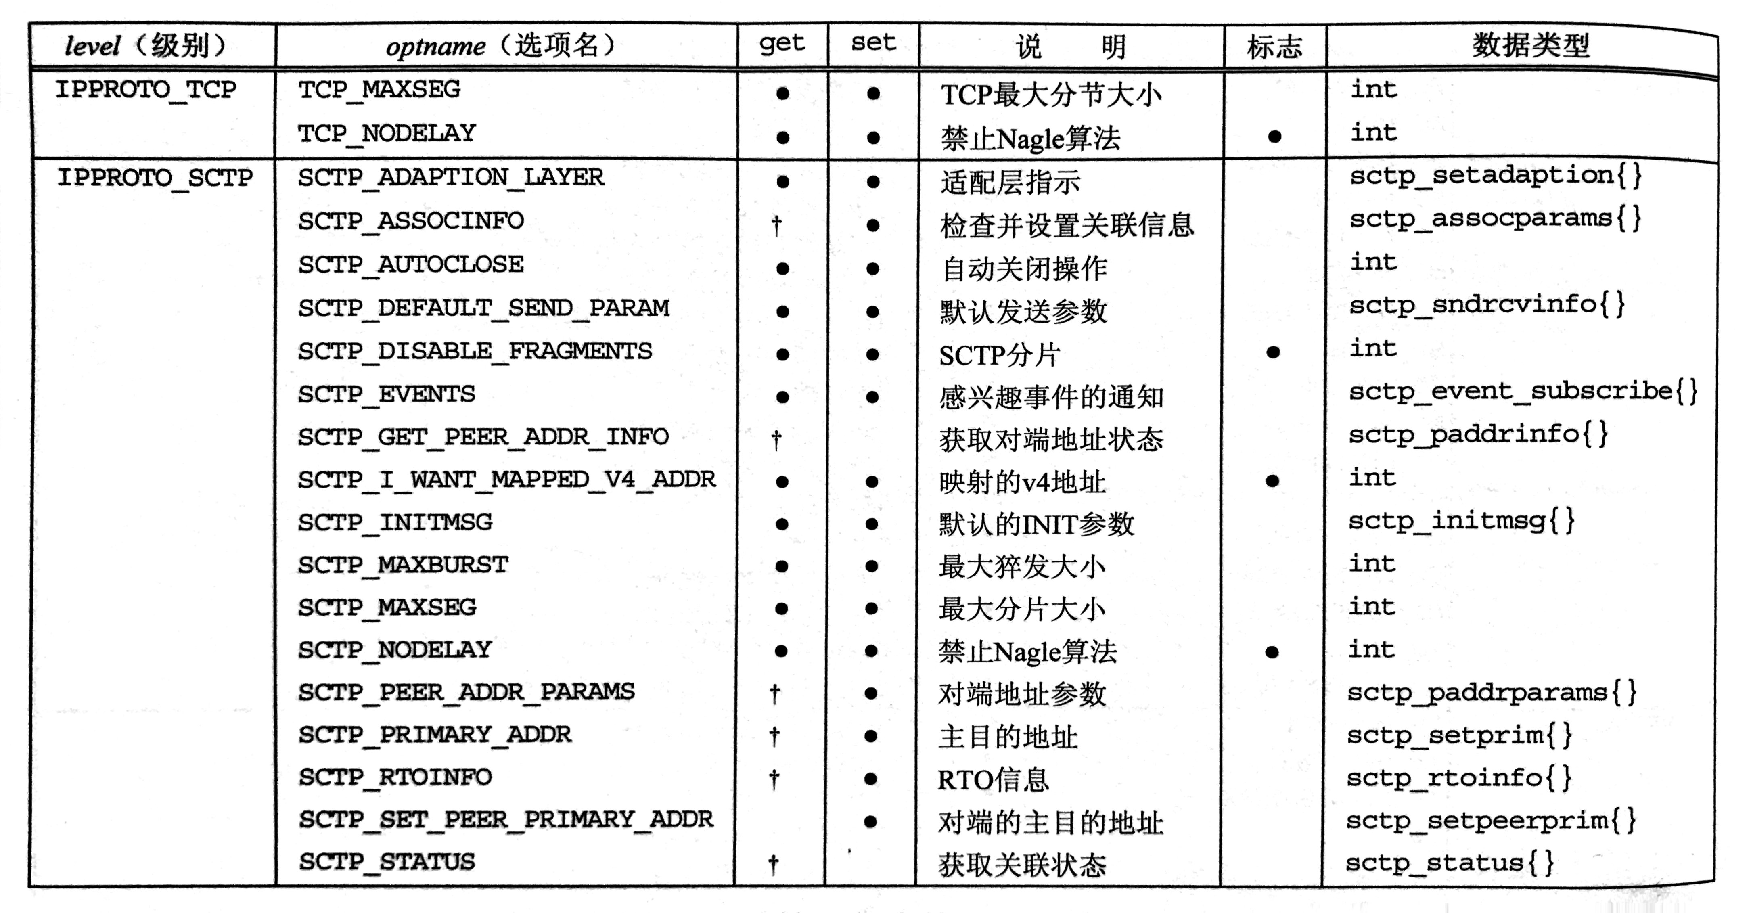
\includegraphics[width=\textwidth]{Picture/getsockopt2}
\end{figure}
\newpage
\begin{figure}[!htb]
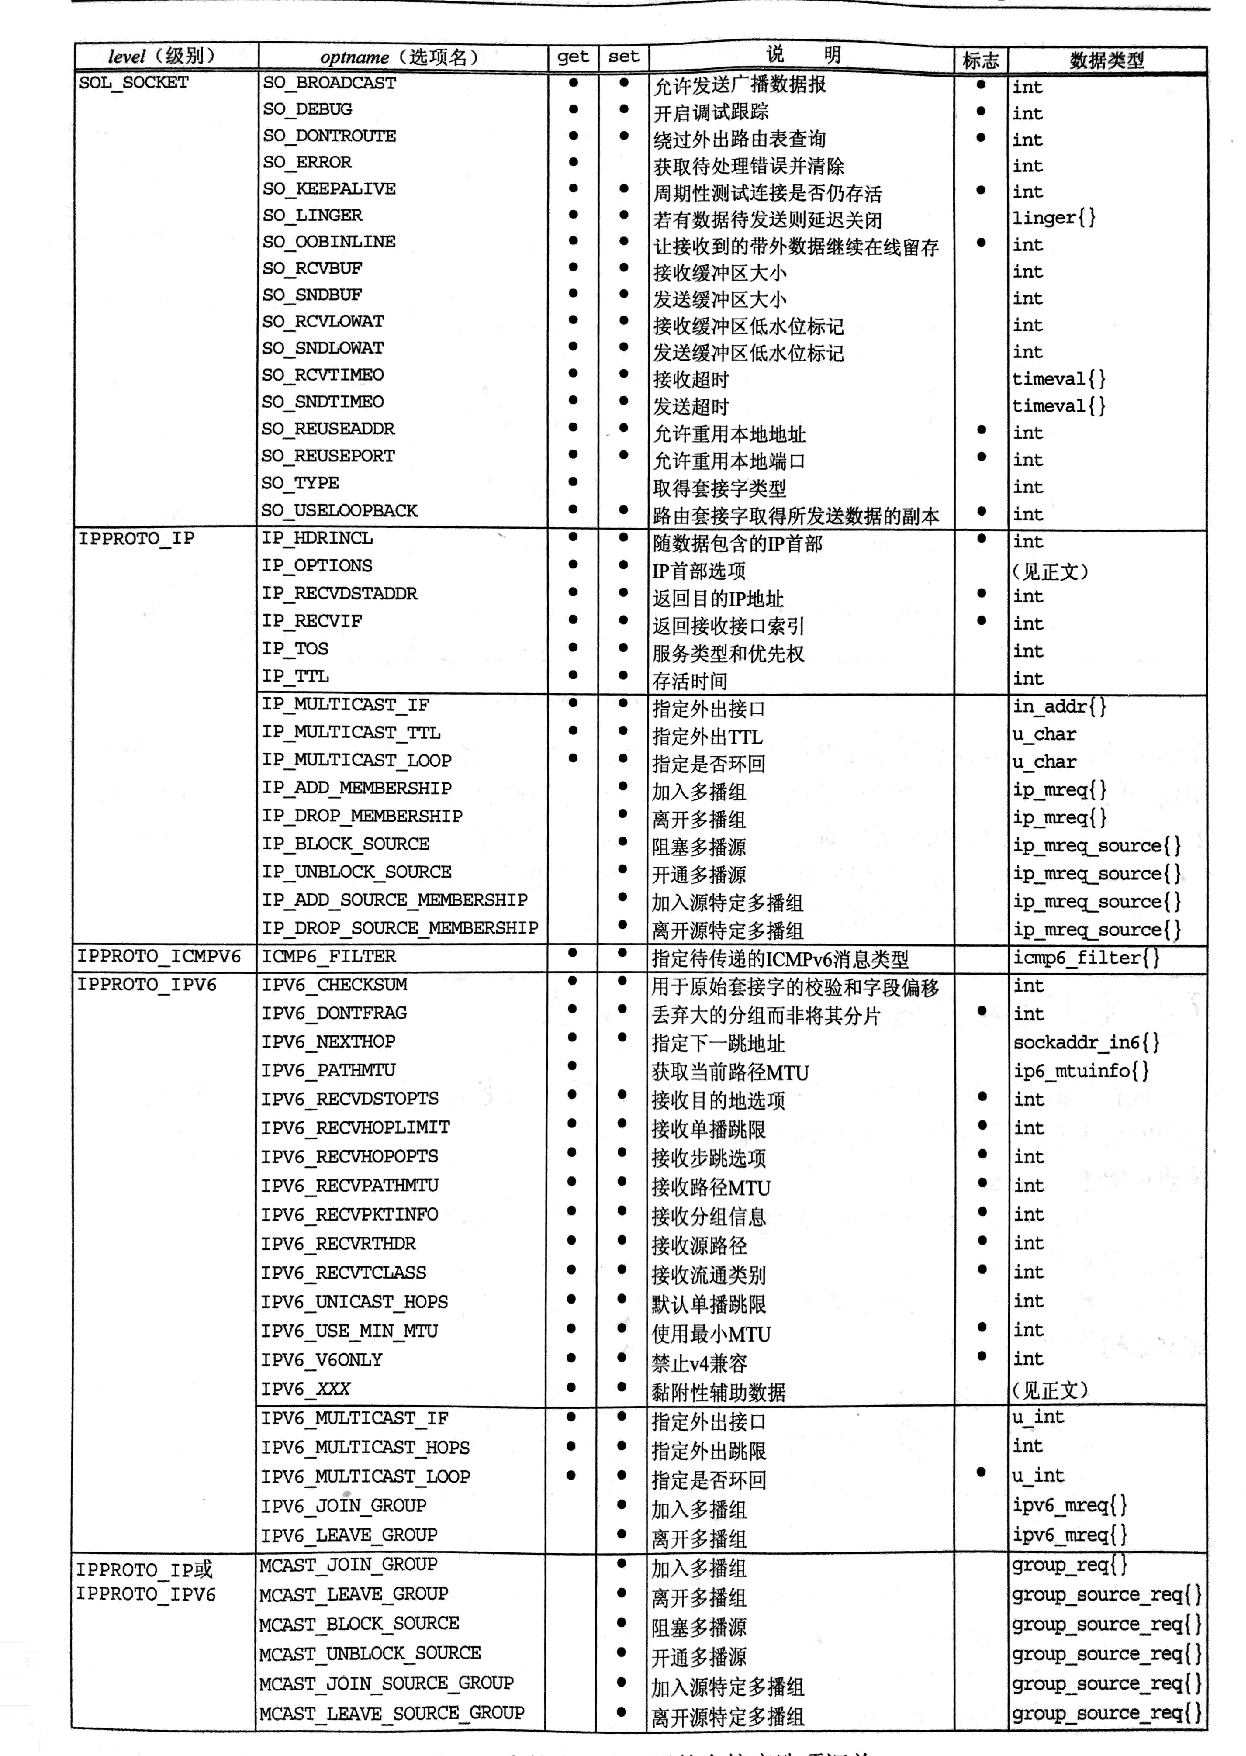
\includegraphics[width=\textwidth]{Picture/getsockopt}
\end{figure}
\end{spacing}
\newpage

\subsection{setsockopt}
\mint[linenos=false]{c}|int setsockopt(int sockfd, int level, int optname, const void *optval, socklen_t optlen);|
\noindent \textbf{设置套接字选项}
\newpage

\subsection{fcntl}
\mint[linenos=false]{c}|int fcntl(int fd, int cmd, ...);|
\noindent \textbf{文件描述符控制}
\begin{spacing}{2.0}
\begin{table}[!htb]
	\begin{tabular}{|c|c|}
	\hline
		F\_SETFL & 设置文件状态标示(全局文件打开表中,可设置O\_XXX) \\
	\hline
		F\_SETOWN & 设置描述符属主 \\
	\hline
		F\_SETFD & 设置文件描述符标志(进程文件描述符表中,FD\_CLOEXEC标志)\\
	\hline
		F\_DUPDF & 复制文件描述符但不会复制FD\_CLOEXEC标志\\
	\hline
		F\_DUPDF\_CLOEXEC & 复制文件描述符但会复制FD\_CLOEXEC标志 \\
	\hline
	\end{tabular}
\end{table}
\begin{minted}[linenos=false]{c}
fcntl(fd, F_SETOWN, pid) //设置接收SIGIO的进程,不能对终端设备使用
fcntl(fd, F_SETFL, flags|O_ASYNC) //设置信号IO
\end{minted} 
\end{spacing}
\newpage

\subsection{readv}
\mint[linenos=false]{c}|ssize_t readv(int fd, const struct iovec *iov, int iovcnt);|
\noindent \textbf{散布读}
\begin{spacing}{2.0}
iovec * 指向一个数组结构,len表示数组长度,从fd读取数据,按iovec数组下标从小到大读取数据到数组元素中所指向的缓冲区中,也就是说如果iovec[0]指向的缓冲区装满后,然后存入iovec[1]指向的缓冲区
\end{spacing}
\newpage

\subsection{writev}
\mint[linenos=false]{c}|ssize_t writev(int fd, const struct iovec *iov, int iovcnt);|
\noindent \textbf{聚集写}
\begin{spacing}{2.0}
向fd写数据,按iovec数组下标从小到大写缓冲区的iov\li len个数据到fd中,也就是说如果iovec[0]指向的缓冲区写到fd后,然后写入iovec[1]指向的缓冲区,如果自己要设置某种信息协议,比如发送的数据以某特定数据开头,特定数据结尾,则此时可以设置三个iovec,分别用于头部数据,中间数据,尾部数据
\end{spacing}
\newpage

\subsection{recvfrom}
\mint[linenos=false]{c}|ssize_t recvfrom(int sockfd, void *buf, size_t len, int flags, struct sockaddr *src_addr, socklen_t *addrlen);|
\noindent \textbf{在一个套接字上接收数据}
\begin{spacing}{2.0}
前三个参数和read函数一样,第四个参数通常指定为0,第五个参数和第六个参数用于获取发信人的协议地址,类似于acccept的第二和第三个参数,返回值也类似write,一般用于UDP

当对UDP调用connect后,可以使用read,recv或recvmsg进行接受数据,此时只会接受源地址为调用connect时指定的IP地址的UDP包
\end{spacing}
\newpage

\subsection{sendto}
\mint[linenos=false]{c}|ssize_t sendto(int sockfd, const void *buf, size_t len, int flags, const struct sockaddr *dest_addr, socklen_t addrlen);|
\noindent \textbf{在一个套接字上发送数据}
\begin{spacing}{2.0}
前三个参数和write函数一样,第四个参数通常指定为0,第五个参数和第六个参数用于指定发送目的地,类似于bind的第二和第三个参数,区别是指定的是目的主机地址,返回值也类似read,一般用于UDP

通常对于客户端来说,不会对它调用bind函数,对于TCP,在它调用connet函数时会由内核来为它分配一个临时端口号,对于UDP来说,会在它首次调用sendto时由内核为它选择一个临时端口

当对UDP调用connect后,无法使用带地址的sendto,可以使用write或send
\end{spacing}
\newpage

\subsection{recv}
\mint[linenos=false]{c}|ssize_t recv(int sockfd, void *buf, size_t len, int flags);|
\noindent \textbf{在一个套接字上接收数据}
\begin{spacing}{2.0}
前三个参数和read一样,但是可以使用flags参数进行一些控制操作
\end{spacing}
\begin{table}[!htb]
\centering
	\begin{tabular}{|c|c|}
	\hline
	flags & 说明 \\
	\hline
		MSG\_DONTWAIT & 仅本操作非阻塞 \\
	\hline
		MSG\_OOB & 发送或接受带外数据 \\
	\hline	
		MSG\_PEEK & 接受数据并保留副本在缓冲区 \\
	\hline		
		MSG\_WAITALL & 等待所有数据 \\
	\hline
	\end{tabular}
\end{table}
\begin{itemize}
	\item MSG\_DONTWAIT: 本标志在无需打开相应套接字非阻塞标志的前提下,把单个IO操作临时指定为非阻塞,接着执行IO操作,然后关闭非阻塞标志
	\item MSG\_OOB: 对于recv,本标志标明即将读入的是带外数据而不是普通数据
	\item MSG\_PEEK: 本标志适用于recv和recvfrom,它允许我们查看已读取的数据,获取缓冲区中数据的一份副本,不会将数据从缓冲区移除
	\item MSG\_WAITALL: 告知内核不要在尚未读取请求数目的字节之前让一个读操作返回,不过在捕获一个信号,连接被终止,套接字发生一个错误的情况下读函数仍然有可能返回比所请求字节数要少的数据
\end{itemize}
\newpage

\subsection{send}
\mint[linenos=false]{c}|ssize_t send(int sockfd, const void *buf, size_t len, int flags);|
\noindent \textbf{在一个套接字上发送数据}
\begin{spacing}{2.0}
前三个参数和write一样,但是可以使用flags参数进行一些控制操作
\end{spacing}
\begin{table}[!htb]
\centering
	\begin{tabular}{|c|c|}
	\hline
	flags & 说明 \\
	\hline
		MSG\_DONTROUTE & 绕过路由表查找 \\
	\hline
		MSG\_DONTWAIT & 仅本操作非阻塞 \\
	\hline
		MSG\_OOB & 发送或接受带外数据 \\
	\hline
	\end{tabular}
\end{table}
\begin{itemize}
	\item MSG\_DONTROUTE: 本标志告知内核目的主机在某个直接连接的本地网络上,因此无需执行路由表查找,此操作等同于对套接字设置SO\_DONTROUTE,但是SO\_DONTROUTE会对针对该套接字的所有IO操作都执行该特性
	\item MSG\_DONTWAIT: 本标志在无需打开相应套接字非阻塞标志的前提下,把单个IO操作临时指定为非阻塞,接着执行IO操作,然后关闭非阻塞标志
	\item MSG\_OOB: 对于send,本标志标明即将发送带外数据,TCP上只有一个字节大小可以作为代外数据发送
\end{itemize}
\newpage

\subsection{recvmsg}
\mint[linenos=false]{c}|ssize_t recvmsg(int sockfd, struct msghdr *msg, int flags);|
\noindent \textbf{在一个套接字上接受数据}
\begin{spacing}{2.0}
可以看作是使用套接字的readv, 接受数据后,msghdr中的msg\li flags元素的可能值有MSG\_CTRUNC|MSG\_EOR|MSG\_ERRQUEUE|MSG\_OOB|MSG\_TRUNC MSG\_CTRUNC表示控制数据被截断,MSG\_EOR表示接受记录结束符,MSG\_ERRQUEUE表示接受错误信息作为辅助数据,MSG\_OOB表示接受带外数据,MSG\_TRUNC表示一般数据被截断
\end{spacing}
\newpage

\subsection{sendmsg}
\mint[linenos=false]{c}|ssize_t sendmsg(int sockfd, const struct msghdr *msg, int flags);|
\noindent \textbf{在一个套接字上发送数据}
\begin{spacing}{2.0}
可以看作是使用套接字的writev,msghdr.control实际上是一个指向cmsghdr的指针,cmsghdr{socklen\li t cmsg\li len; int cmsg\li level; int cmsg\li type} 为了发送文件描述符,将cmsg\li len设置为cmsghdr结构的长度加一个整形的长度(描述符的长度),cmsg\li level字段设置为SOL\_SOCKET,cmsg\li type设置为SCM\_RIGHTS,用以表明在传送访问权(SCM是套接字级控制信息的缩写),访问权限仅能通过UNIX域套接字发送,描述符仅随cmsg\li type后存储

\end{spacing}
\newpage

\subsection{gethostbyname}
\mint[linenos=false]{c}|struct hostent *gethostbyname(const char *name);|
\noindent \textbf{查询域名服务器,获取一个域名的IP地址信息}
\begin{spacing}{2.0}
虽然说此函数以过时,但是短时间内想要完全废弃时不可能的,此函数只能处理IPv4地址,也就是说只能查询域名服务器里面的A类记录,后面可以使用gethostinfo代替

函数出错时不会设置errno变量,而是会设置h\li errno变量,这个变量设置在netdb.h头文件中

\begin{itemize}
	\item HOST\_NOT\_FOUND
	\item TRY\_AGAIN
	\item NO\_RECOVERY
	\item NO\_DATA
\end{itemize}
大多数系统都提供了一个hstrerrno的函数,它以某个h\li errno值作为一个唯一的参数,返回的是一个const char *指针,指向对应错误的说明
\end{spacing}
\textbf{以下是一个gethostbyname的使用例子}
\begin{minted}{c}
# include </Users/dengyan/ClionProjects/Linux/linux.h>

int main(int argc, char *argv[]) {
    struct hostent * result;
    char buf[100];
    char ** p;

    if((result = gethostbyname("www.baidu.com")) == NULL) {
        printf("%s", hstrerror(h_errno));
        exit(-1);
    }

    p = result->h_aliases;
    while (*p != NULL) {
        printf("%s", *p);
        p++;
    }

    p = result->h_addr_list;
    while (*p != NULL) {
        printf("%s\n", inet_ntop(AF_INET, *p, buf, sizeof(buf)));
        p++;
    }
    return 0;
}
\end{minted}
\newpage

\subsection{gethostbyaddr}
\mint[linenos=false]{c}|struct hostent *gethostbyaddr(const void *addr, socklen_t len, int type);|
\noindent \textbf{使用IP地址查找主机名}
\begin{spacing}{2.0}
功能上与gethostbyname相反,在这里我们所关心的是hostent结构体中的h\li name域
\end{spacing}
\newpage

\subsection{getservbyname}
\mint[linenos=false]{c}|struct servent *getservbyname(const char *name, const char *proto);|
\noindent \textbf{根据服务名和协议名查询信息}
\begin{spacing}{2.0}
使用本地文件/etc/services

name表示服务名,proto表示协议名,根据服务名(如ssh)和协议名(如tcp)查询信息,这里主要关注的是端口信息
\end{spacing}
\newpage

\subsection{getservbyport}
\mint[linenos=false]{c}|struct servent *getservbyport(int port, const char *proto);|
\noindent \textbf{根据端口号和协议名查询信息}
\begin{spacing}{2.0}
使用本地文件/etc/services

port表示端口号,proto表示协议名,根据端口名(如23,需要使用网络序)和协议名(tcp)查询信息

\begin{minted}{c}
/* 三个相关函数 */
struct servent *getservent(void); //获取文件下一条目
void setservent(int stayopen); //打开端口绑定的服务名和端口号信息文件,mac上即/etc/services文件
void endservent(void); //关闭文件
\end{minted}
\end{spacing}
\newpage

\subsection{getaddrinfo}
\mint[linenos=false]{c}|int getaddrinfo(const char *node, const char *service, const struct addrinfo *hints, struct addrinfo **res);|
\noindent \textbf{进行域名到IP以及服务名到端口号的转换}
\begin{spacing}{2.0}
等价于一个支持IPv6的gethostbyname加getservbyname之和

node参数即可与为域名,也可以为点分十进制字符串

hints用于暗示返回的值,返回值将由res指向,也就是说传入的res参数是是一个指针变量的地址

UNP p249
\end{spacing}

\textbf{以下是几个getaddrinfo的借口函数}
\subsubsection{host\li serv}
\begin{minted}{c}
struct addrinfo * host_serv(const char * host, const char * serv, int family, int socktype)
{
    struct addrinfo hints, *res;

    bzero(&hints, sizeof(struct addrinfo));
    hints.ai_flags = AI_CANONNAME;
    hints.ai_family = family;
    hints.ai_socktype = socktype;

    if (getaddrinfo(host, serv, &hints, &res) != 0)
        return  NULL;
    return res;
}
\end{minted}

\newpage
\subsubsection{tcp\li connect}
\begin{minted}{c}
int tcp_connect(const char * host, const char * serv)
{
    int sockfd, n;
    struct addrinfo hints, *res, *ressave;

    bzero(&hints, sizeof(struct addrinfo));
    hints.ai_family = AF_UNSPEC;
    hints.ai_socktype = SOCK_STREAM;
    hints.ai_flags = AI_NUMERICSERV;

    if ((n = getaddrinfo(host, serv, &hints, &res)) != 0)
        err_quit("tcp_connect error for %s, %s:%s", host, serv, gai_strerror(n));

    ressave = res;
    do {
        sockfd = socket(res->ai_family, res->ai_socktype, res->ai_protocol);
        if (sockfd < 0)
            continue;

        if (connect(sockfd, res->ai_addr, res->ai_addrlen) == 0)
            break;

        close(sockfd);
    } while ((res = res->ai_next) != NULL);

    if (res == NULL)
        err_quit("tcp_connect error for %s, %s", host, serv);

    freeaddrinfo(ressave);

    return sockfd;
}
\end{minted}
\newpage

\subsubsection{tcp\li connect}
\begin{minted}{c}
int tcp_listen(const char * host, const char * serv, socklen_t * addrlenp)
{
    int listenfd, n;
    const int on = 1;
    struct addrinfo hints, *res, *ressave;

    bzero(&hints, sizeof(struct addrinfo));
    hints.ai_flags = AI_PASSIVE;
    hints.ai_family = AF_UNSPEC;
    hints.ai_socktype = SOCK_STREAM;
    hints.ai_flags = AI_NUMERICSERV;

    if ((n = getaddrinfo(host, serv, &hints, &res)) != 0)
        err_quit("tcp_listen error for %s, %s:%s", host, serv, gai_strerror(n));
    ressave = res;
    do {
        listenfd = socket(res->ai_family, res->ai_socktype, res->ai_protocol);
        if (listenfd < 0)
            continue;

        setsockopt(listenfd, SOL_SOCKET, SO_REUSEADDR, &on, sizeof(on));
        if (bind(listenfd, res->ai_addr, res->ai_addrlen) == 0)
            break;

        close(listenfd);
    } while ((res = res->ai_next) != NULL);

    listen(listenfd, 5);
    if (addrlenp)
        *addrlenp = res->ai_addrlen;

    return listenfd;
}
\end{minted}
\newpage

\subsection{gai\li strerror}
\mint[linenos=false]{c}|const char *gai_strerror(int errcode);|
\noindent \textbf{如果getaddrinfo失败,使用此函数将getaddrinfo的返回值转换成错误信息}
\newpage

\subsection{freeaddrinfo}
\mint[linenos=false]{c}|void freeaddrinfo(struct addrinfo *res);|
\noindent \textbf{释放getaddrinfo第四个参数指向的addrinfo结构}
\newpage

\subsection{getnameinfo}
\mint[linenos=false]{c}|int getnameinfo(const struct sockaddr *addr, socklen_t addrlen, char *host, socklen_t hostlen, char *serv, socklen_t servlen, int flags);|
\noindent \textbf{根据套接字地址获取主机名和服务名}

\begin{table}[!htb]
\centering
	\begin{tabular}{|c|c|}
	\hline
	常值 & 说明 \\
	\hline
	NI\_DGRAM & 数据报服务 \\
	\hline
	NI\_NAMEREQD & 若不能从地址解析出名字则返回错误 \\
	\hline
	NI\_NOFQDN & 只返回FQDN的主机名部分 \\
	\hline
	NI\_NUMERICHOST & 以数字串格式返回主机字符串 \\
	\hline
	NI\_NUMERICSCOPE & 以数字串格式返回范围表示标示字符串 \\
	\hline
	NI\_NUMERICSERV & 以数字串格式返回服务字符串 \\
	\hline
	\end{tabular}
	\caption{getnameinfo的标志值}
\end{table}
\newpage

\subsection{}
\mint[linenos=false]{c}||
\noindent \textbf{}
\begin{spacing}{2.0}

\end{spacing}
\newpage

\newpage

\section{{\color[rgb]{0.2,0.4,0.6}例子}}
\subsection{时间客户端及服务器端}
\subsubsection{客户端}
\begin{minted}{c}
# include </Users/dengyan/ClionProjects/Linux/linux.h>

int main(int argc, char *argv[]) {
    int sockfd, n;
    char buf[4097];
    struct sockaddr_in servaddr;

    if ((sockfd = socket(AF_INET, SOCK_STREAM, 0)) == -1)
        err_sys("socket error");

    bzero(&servaddr, sizeof(servaddr));
    servaddr.sin_family = AF_INET;
    servaddr.sin_port = htons(13333);
    if (inet_pton(AF_INET, "127.0.0.1", &servaddr.sin_addr) == -1)
        err_quit("inet_pton error");

    if (connect(sockfd, (struct sockaddr *)&servaddr, sizeof(servaddr)) < 0)
        err_sys("connect error");

    while ((n = read(sockfd, buf, 4096)) > 0) {
        write(STDOUT_FILENO, buf, n);
    }
    return 0;
}
\end{minted}
\subsubsection{服务器端}
\begin{minted}{c}
# include </Users/dengyan/ClionProjects/Linux/linux.h>

int main(int argc, char *argv[]) {
    int sockfd, n, fd;
    struct sockaddr_in servaddr;

    if ((sockfd = socket(AF_INET, SOCK_STREAM, 0)) < 0)
        exit(-1);

    bzero(&servaddr, sizeof(servaddr));
    servaddr.sin_port = htons(13333);
    servaddr.sin_family = AF_INET;
    if (inet_pton(AF_INET, "127.0.0.1", &servaddr.sin_addr) <= 0)
        exit(-1);

    if (bind(sockfd, (struct sockaddr *)&servaddr, sizeof(servaddr)) != 0) {
        exit(-1);
    }

    listen(sockfd, 5);

    while (1) {
        if ((fd = accept(sockfd, NULL, NULL)) < 0) {
            printf("%s", strerror(errno));
            continue;
        }
        time_t t = time(NULL);
        char * str = ctime(&t);
        write(fd, str, strlen(str));
        close(fd);
    }

}
\end{minted}
\newpage

\subsection{使用select实现的echo服务器(TCP及UDP同时支持)}
\subsubsection{客户端}
\begin{minted}{c}
# include </Users/dengyan/ClionProjects/Linux/linux.h>

int main(int argc, char *argv[]) {
    char buf[4096];
    int tcpfd, udpfd, len, choose, n;
    struct sockaddr_in servaddr, cliaddr;

    if ((tcpfd = socket(AF_INET, SOCK_STREAM, 0)) < 0)
        err_sys("tcp socket error");

    bzero(&servaddr, sizeof(servaddr));
    servaddr.sin_family = AF_INET;
    servaddr.sin_port = htons(23333);
    servaddr.sin_addr.s_addr = htonl(INADDR_LOOPBACK);

    if ((udpfd = socket(AF_INET, SOCK_DGRAM, 0)) < 0)
        err_sys("udp socket error");

    if (connect(tcpfd, (struct sockaddr *)&servaddr, sizeof(servaddr)) < 0)
        err_sys("connect error");


    connect(udpfd, (struct sockaddr *)&servaddr, sizeof(servaddr));

    for (;;) {
        printf("1: TCP echo\n");
        printf("2: UDP echo\n");

        scanf("%d", &choose);
        switch (choose) {
            case 1:
                n = read(STDIN_FILENO, buf, 4096);
                write(tcpfd, buf, n);
                n = read(tcpfd, buf, n);
                write(STDOUT_FILENO, buf, n);
                break;
            case 2:
                n = read(STDIN_FILENO, buf, 4096);
                write(udpfd, buf, n);
                n = read(udpfd, buf, n);
                write(STDOUT_FILENO, buf, n);
                break;
            default:
                break;
        }
    }

    return 0;
}
\end{minted}

\subsubsection{服务器端}
\begin{minted}{c}
# include </Users/dengyan/ClionProjects/Linux/linux.h>

void handler(int s)
{
    pid_t pid;
    while ((pid = waitpid(-1, NULL, WNOHANG)) > 0)
        printf("child pid %d terminate ", pid);
}

int main(int argc, char *argv[]) {
    int listenfd, clifd, udpfd, n;
    socklen_t len;
    int on = 1, maxfd = -1;
    struct sockaddr_in servaddr, cliaddr;

    if ((listenfd = socket(AF_INET, SOCK_STREAM, 0)) < 0)
        err_quit("socket error");

    bzero(&servaddr, sizeof(servaddr));
    servaddr.sin_family = AF_INET;
    servaddr.sin_port = htons(23333);
    servaddr.sin_addr.s_addr = htonl(INADDR_ANY);

    signal(SIGCHLD, handler);
    
    if (setsockopt(listenfd, SOL_SOCKET, SO_REUSEADDR, &on, sizeof(on)) == -1)
        err_quit("setsockopt error");
    
    if (bind(listenfd, (struct sockaddr *)&servaddr, sizeof(servaddr)) < 0)
        err_quit("bind error");

    listen(listenfd, 5);

    if ((udpfd = socket(AF_INET, SOCK_DGRAM, 0)) < 0)
        err_quit("udp socket error");

    if (bind(udpfd, (struct sockaddr *)&servaddr, sizeof(servaddr)) < 0)
        err_quit("bind error");

    maxfd = listenfd > udpfd?listenfd:udpfd;
    fd_set set;
    FD_ZERO(&set);

    for ( ;; ) {
        FD_SET(listenfd, &set);
        FD_SET(udpfd, &set);

        if (select(maxfd + 1, &set, NULL, NULL, NULL) < 0) {
            if (errno == EINTR)
                continue;
            else
                err_sys("select error");
        }

        if (FD_ISSET(listenfd, &set)) {
            char name[40];
            len = sizeof(cliaddr);
            clifd = accept(listenfd, (struct sockaddr *)&cliaddr, &len);
            printf("connect from %s:%d\n", inet_ntop(AF_INET, &cliaddr.sin_addr, name, sizeof(name)), ntohs(cliaddr.sin_port));
            fflush(stdout);

            if (fork() == 0) {
                char buf[4096];
                close(listenfd);
                while ((n = read(clifd, buf, sizeof(buf))) > 0) {
                    write(clifd, buf, n);
                }
                exit(-1);
            }
            close(clifd);
        }

        if (FD_ISSET(udpfd, &set)) {
            char buf[4096];
            len = sizeof(cliaddr);
            n = recvfrom(udpfd, buf, sizeof(buf), 0, (struct sockaddr *)&cliaddr, &len);
            sendto(udpfd, buf, n, 0, (struct sockaddr *)&cliaddr, len);
        }
    }
}
\end{minted}
\newpage

\subsection{使用getaddrinfo基于tcp实现的时间服务器}
\subsubsection{客户端}
\begin{minted}{c}
# include </Users/dengyan/ClionProjects/Linux/linux.h>

int main(int argc, char *argv[]) {
    int sockfd, n;
    char buf[100];
    char recvline[MAXLINE + 1];
    socklen_t len;
    struct sockaddr_storage ss;

    sockfd = tcp_connect("localhost", "13333");
    len = sizeof(ss);
    getpeername(sockfd, (struct sockaddr *)&ss, &len);
    printf("connected to %s\n", len==16?inet_ntop(AF_INET, &((struct sockaddr_in *)&ss)->sin_addr, buf, 100):inet_ntop(AF_INET6, &((struct sockaddr_in *)&ss)->sin_addr, buf, 100));

    while ((n = read(sockfd, recvline, MAXLINE)) > 0) {
        write(STDOUT_FILENO, recvline, n);
    }
    return 0;
}
\end{minted}

\subsubsection{服务器端}
\begin{minted}{c}
# include </Users/dengyan/ClionProjects/Linux/linux.h>

int main(int argc, char *argv[]) {
    int listenfd, connfd;
    socklen_t len;
    char buf[MAXLINE];
    time_t t;
    struct sockaddr_storage cliaddr;

    listenfd = tcp_listen(NULL, "13333", NULL);

    for ( ;; ) {
        len = sizeof(cliaddr);
        connfd = accept(listenfd, (struct sockaddr *)&cliaddr, &len);
        printf("connected to %s\n", len==16?inet_ntop(AF_INET, &((struct sockaddr_in *)&cliaddr)->sin_addr, buf, 100):inet_ntop(AF_INET6, &((struct sockaddr_in *)&cliaddr)->sin_addr, buf, 100));

        t = time(NULL);
        char * s = ctime(&t);
        write(connfd, s, strlen(s));
        close(connfd);
    }
    return 0;
}
\end{minted}
\newpage

\subsection{观察TCP阻塞窗口}
\subsubsection{客户端}
\begin{minted}{c}
# include </Users/dengyan/ClionProjects/Linux/linux.h>

int main(int argc, char *argv[]) {
    int fd, n;
    char buf[MAXLINE];
    struct sockaddr_in servaddr;
    struct tcp_connection_info tcpinfo;
    int len = sizeof(tcpinfo);
    fd = socket(AF_INET, SOCK_STREAM, 0);

    int sfd = open("/dev/zero", O_RDONLY);
    read(sfd, buf, 1000);

    bzero(&servaddr, sizeof(servaddr));
    servaddr.sin_port = htons(23333);
    servaddr.sin_family = AF_INET;
    servaddr.sin_addr.s_addr = htonl(INADDR_LOOPBACK);

    connect(fd, &servaddr, sizeof(servaddr));
    printf("接收窗口 发送窗口 发送阻塞窗口\n");
    while (write(fd, buf, 1000) > 0)
    {
        getsockopt(fd, IPPROTO_TCP, TCP_CONNECTION_INFO, &tcpinfo, &len);
        printf("%d %d %d\n", tcpinfo.tcpi_rcv_wnd, tcpinfo.tcpi_snd_wnd, tcpinfo.tcpi_snd_cwnd);
        sleep(0.2);
    }
}
\end{minted}

\subsubsection{服务器端}
\begin{minted}{c}
# include </Users/dengyan/ClionProjects/Linux/linux.h>

int main(int argc, char *argv[]) {
    setbuf(stdout, NULL);
    int listenfd, n = 4;
    int rcv = 0;
    char buf[MAXLINE];
    struct tcp_connection_info tcpinfo;
    int len = sizeof(tcpinfo);

    struct addrinfo hints, *res, *ressave;

    bzero(&hints, sizeof(hints));
    hints.ai_family = AF_INET;
    hints.ai_socktype = SOCK_STREAM;
    hints.ai_flags = AI_PASSIVE|AI_NUMERICSERV;

    if (getaddrinfo(NULL, "23333", &hints, &res) != 0)
        err_quit("getaddrinfo error");

    ressave = res;
    do {
        listenfd = socket(AF_INET, SOCK_STREAM, 0);

        setsockopt(listenfd, SOL_SOCKET, SO_REUSEADDR, &n, sizeof(int));

        if (bind(listenfd, res->ai_addr, res->ai_addrlen) == 0)
            break;

        close(listenfd);
    } while ((res = res->ai_next) != NULL);

    if (res == NULL)
        err_quit("don't find the socket to bind");

    freeaddrinfo(ressave);

    getsockopt(listenfd, SOL_SOCKET, SO_RCVBUF, &rcv, &n);
    printf("rcvbuf = %d\n", rcv);
    rcv = 262000;
    setsockopt(listenfd, SOL_SOCKET, SO_RCVBUF, &rcv, n);
    printf("rcvbuf = %d\n", rcv);
    listen(listenfd, 5);

    int fd = accept(listenfd, NULL, 0);
    printf("接收窗口 发送窗口 发送阻塞窗口\n");

    for (;;) {
        getsockopt(fd, IPPROTO_TCP, TCP_CONNECTION_INFO, &tcpinfo, &len);
        printf("%d %d %d\n", tcpinfo.tcpi_rcv_wnd, tcpinfo.tcpi_snd_wnd, tcpinfo.tcpi_snd_cwnd);
        sleep(1);
    }
    return 0;
}
\end{minted}

\subsection{XX}
\subsubsection{客户端}
\begin{minted}{c}

\end{minted}

\subsubsection{服务器端}
\begin{minted}{c}

\end{minted}



\newpage

\section{{\color[rgb]{0.2,0.4,0.6}结构体}}
\subsection{netinet/in.h}
\subsubsection{in\li addr}
\begin{minted}{c}
struct in_addr {
    in_addr_t s_addr; //IPv4地址,通常为uint32_t
};
/*
 * 需要注意的是,对32位IPv4地址进行访问时有两种不同的访问方法
 * 一种是访问结构体,另一种是访问结构体中的成员
 * 在当中参数时需要小心处理,因为编译器处理结构体和
 * 无符号整形采用不同的方式,结构体作为左值时无法随意赋值
 * 所以如果想直接对地址赋值需要访问结构体中的成员
 */
\end{minted}

\subsubsection{sockaddr\li in}
\begin{minted}{c}
struct sockaddr_in {
    __uint8_t   sin_len; //通常不需要设置和检查
    sa_family_t sin_family; //地址族(AF_INET),通常为8位的无符号整形
    in_port_t   sin_port; //TCP或UDP端口,一般为uint16_t
    struct in_addr sin_addr; //IPv4地址,通常为uint32_t
    char        sin_zero[8]; //用于填充,达到最小16个字节
};
\end{minted}

\subsubsection{in6\li addr}
\begin{minted}{c}
//此结构在mac上为<netinet6/in6.h>中
typedef struct in6_addr {
    union {
        __uint8_t   __u6_addr8[16];
        __uint16_t  __u6_addr16[8];
        __uint32_t  __u6_addr32[4];
    } __u6_addr; /* 128-bit IP6 address */
} in6_addr_t;
//通配地址赋值给此结构体可以使用in6_addr = in6addr_any
\end{minted}

\subsubsection{sockaddr\li in6}
\begin{minted}{c}
//此结构在mac上为<netinet6/in6.h>中
struct sockaddr_in6 {
    __uint8_t   sin6_len; //通常不需要设置和检查
    sa_family_t sin6_family; //地址族(AF_INET6)
    in_port_t   sin6_port;
    __uint32_t  sin6_flowinfo;
    struct in6_addr	sin6_addr;
    __uint32_t  sin6_scope_id;
};
\end{minted}

\subsection{sys/socket.h}
\subsubsection{sockaddr}
\begin{minted}{c}
//16个字节,不足以容纳容纳IPv6结构
struct sockaddr {
    __uint8_t    sa_len;
    sa_family_t sa_family;
    char        sa_data[14];
};
\end{minted}

\subsubsection{sockaddr\li storage}
\begin{minted}{c}
/*
 * 由于sockaddr不足以容纳所有的地址结构,所以新的通用套接字结构产生了
 * 它足以容纳所有类型的套接字地址结构,而且满足最苛刻的对齐要求
 * 但是需要将其转换为特定的类型后,才可以访问其内部字段
 */
struct sockaddr_storage {
    __uint8_t   ss_len;
    sa_family_t ss_family;
    char        __ss_pad1[_SS_PAD1SIZE];
    __int64_t   __ss_align;
    char        __ss_pad2[_SS_PAD2SIZE];
};
\end{minted}

\subsubsection{iovec}
\begin{minted}{c}
struct iovec {
    void  *iov_base;    /* 缓冲区地址 */
    size_t iov_len;     /* 缓冲区有效数据长度 */
};
\end{minted}

\subsubsection{msghdr}
\begin{minted}{c}
struct msghdr {
    void         *msg_name;       /* 地址 */
    socklen_t     msg_namelen;    /* 地址长度 */
    struct iovec *msg_iov;        /* 用于散步读聚集写的数组 */
    size_t        msg_iovlen;     /* 数组长度 */
    void         *msg_control;    /* 指向控制信息头 */
    size_t        msg_controllen; /* 控制信息大小 */
    int           msg_flags;      /* 标志 */
};
\end{minted}

\subsection{netdb.h}
\subsubsection{hostent}
\begin{minted}{c}
struct hostent {
    char  *h_name;            /* 正式主机名 */
    char **h_aliases;         /* 别名列表 */
    int    h_addrtype;        /* 主机地址类型: AF_INET */
    int    h_length;          /* 地址长度: 4 */
    char **h_addr_list;       /* 其中的每个指针指向in_addr结构体 */
}
\end{minted}

\subsubsection{servent}
\begin{minted}{c}
struct servent {
    char  *s_name;       /* 正式服务名 */
    char **s_aliases;    /* 别名列表 */
    int    s_port;       /* 端口号(网络序) */
    char  *s_proto;      /* 使用的协议名 */
}
\end{minted}

\subsubsection{addrinfo}
\begin{minted}{c}
struct addrinfo {
    int              ai_flags; /* 控制返回信息 */
    int              ai_family; /* AF_INET|AF_INET6|AF_UNSPEC 意义为获取哪种地址结构 */
    int              ai_socktype; /* SOCK_XXX */
    int              ai_protocol; /* 一般为0 */
    socklen_t        ai_addrlen; /* ai_addr长度 */
    struct sockaddr *ai_addr; /* 存放地址信息 */
    char            *ai_canonname;
    struct addrinfo *ai_next; /* 指向链表上的下一个addrinfo */
};

/* ------------ai_flags------------
 * AI_PASSIVE 套接字将用于被动打开(服务器端)
 * AI_CANONNAME 告知getaddrinfo返回主机的规范名字
 * AI_V4MAPPED 如果ai_family指定的是IPv6,那么如果没有可用的AAAA记录,则返回一条IPv4映射的IPv6地址)
 * AI_ADDRCONFIG表示按照主机配置配置选择返回的地址类型
 * AI_ALL表示查找IPv4和IPv6(IPv6需要指定AI_V4MAPPED后还会返回IPv4映射的IPv6地址)
 * AI_NUMERICHOST表示以数字格式指定主机地址
 * AI_NUMERICSERV表示以数字形式(端口号)指定服务
 */
\end{minted}

\end{document}
